% Created by tikzDevice version 0.12.6 on 2026-05-14 21:46:37
% !TEX encoding = UTF-8 Unicode
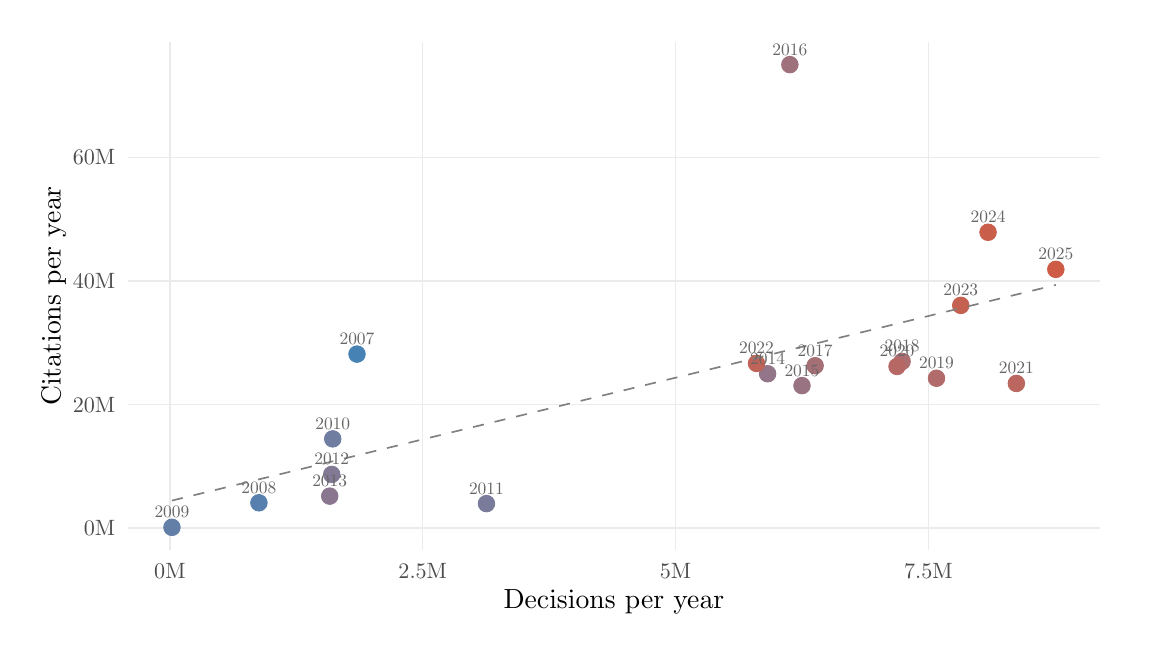
\begin{tikzpicture}[x=1pt,y=1pt]
\definecolor{fillColor}{RGB}{255,255,255}
\path[use as bounding box,fill=fillColor,fill opacity=0.00] (0,0) rectangle (397.48,216.81);
\begin{scope}
\path[clip] (  0.00,  0.00) rectangle (397.48,216.81);
\definecolor{fillColor}{RGB}{255,255,255}

\path[fill=fillColor] ( -0.00,  0.00) rectangle (397.48,216.81);
\end{scope}
\begin{scope}
\path[clip] ( 36.16, 27.90) rectangle (387.48,211.81);
\definecolor{drawColor}{gray}{0.92}

\path[draw=drawColor,line width= 0.5pt,line join=round] ( 36.16, 35.99) --
	(387.48, 35.99);

\path[draw=drawColor,line width= 0.5pt,line join=round] ( 36.16, 80.66) --
	(387.48, 80.66);

\path[draw=drawColor,line width= 0.5pt,line join=round] ( 36.16,125.32) --
	(387.48,125.32);

\path[draw=drawColor,line width= 0.5pt,line join=round] ( 36.16,169.99) --
	(387.48,169.99);

\path[draw=drawColor,line width= 0.5pt,line join=round] ( 51.40, 27.90) --
	( 51.40,211.81);

\path[draw=drawColor,line width= 0.5pt,line join=round] (142.76, 27.90) --
	(142.76,211.81);

\path[draw=drawColor,line width= 0.5pt,line join=round] (234.11, 27.90) --
	(234.11,211.81);

\path[draw=drawColor,line width= 0.5pt,line join=round] (325.47, 27.90) --
	(325.47,211.81);
\definecolor{drawColor}{RGB}{70,130,180}
\definecolor{fillColor}{RGB}{70,130,180}

\path[draw=drawColor,line width= 0.3pt,line join=round,line cap=round,fill=fillColor] (119.00, 98.86) circle (  3.00);
\definecolor{drawColor}{RGB}{87,128,174}
\definecolor{fillColor}{RGB}{87,128,174}

\path[draw=drawColor,line width= 0.3pt,line join=round,line cap=round,fill=fillColor] ( 83.56, 45.12) circle (  3.00);
\definecolor{drawColor}{RGB}{100,127,167}
\definecolor{fillColor}{RGB}{100,127,167}

\path[draw=drawColor,line width= 0.3pt,line join=round,line cap=round,fill=fillColor] ( 52.13, 36.26) circle (  3.00);
\definecolor{drawColor}{RGB}{111,125,161}
\definecolor{fillColor}{RGB}{111,125,161}

\path[draw=drawColor,line width= 0.3pt,line join=round,line cap=round,fill=fillColor] (110.23, 68.22) circle (  3.00);
\definecolor{drawColor}{RGB}{121,123,155}
\definecolor{fillColor}{RGB}{121,123,155}

\path[draw=drawColor,line width= 0.3pt,line join=round,line cap=round,fill=fillColor] (165.78, 44.83) circle (  3.00);
\definecolor{drawColor}{RGB}{130,121,149}
\definecolor{fillColor}{RGB}{130,121,149}

\path[draw=drawColor,line width= 0.3pt,line join=round,line cap=round,fill=fillColor] (109.87, 55.37) circle (  3.00);
\definecolor{drawColor}{RGB}{138,119,143}
\definecolor{fillColor}{RGB}{138,119,143}

\path[draw=drawColor,line width= 0.3pt,line join=round,line cap=round,fill=fillColor] (109.14, 47.53) circle (  3.00);
\definecolor{drawColor}{RGB}{146,117,136}
\definecolor{fillColor}{RGB}{146,117,136}

\path[draw=drawColor,line width= 0.3pt,line join=round,line cap=round,fill=fillColor] (267.37, 91.76) circle (  3.00);
\definecolor{drawColor}{RGB}{153,115,130}
\definecolor{fillColor}{RGB}{153,115,130}

\path[draw=drawColor,line width= 0.3pt,line join=round,line cap=round,fill=fillColor] (279.79, 87.47) circle (  3.00);
\definecolor{drawColor}{RGB}{159,113,124}
\definecolor{fillColor}{RGB}{159,113,124}

\path[draw=drawColor,line width= 0.3pt,line join=round,line cap=round,fill=fillColor] (275.41,203.45) circle (  3.00);
\definecolor{drawColor}{RGB}{165,111,118}
\definecolor{fillColor}{RGB}{165,111,118}

\path[draw=drawColor,line width= 0.3pt,line join=round,line cap=round,fill=fillColor] (284.54, 94.66) circle (  3.00);
\definecolor{drawColor}{RGB}{171,109,112}
\definecolor{fillColor}{RGB}{171,109,112}

\path[draw=drawColor,line width= 0.3pt,line join=round,line cap=round,fill=fillColor] (315.97, 96.20) circle (  3.00);
\definecolor{drawColor}{RGB}{177,107,106}
\definecolor{fillColor}{RGB}{177,107,106}

\path[draw=drawColor,line width= 0.3pt,line join=round,line cap=round,fill=fillColor] (328.40, 90.13) circle (  3.00);
\definecolor{drawColor}{RGB}{182,104,100}
\definecolor{fillColor}{RGB}{182,104,100}

\path[draw=drawColor,line width= 0.3pt,line join=round,line cap=round,fill=fillColor] (314.14, 94.39) circle (  3.00);
\definecolor{drawColor}{RGB}{187,102,94}
\definecolor{fillColor}{RGB}{187,102,94}

\path[draw=drawColor,line width= 0.3pt,line join=round,line cap=round,fill=fillColor] (357.26, 88.25) circle (  3.00);
\definecolor{drawColor}{RGB}{192,99,88}
\definecolor{fillColor}{RGB}{192,99,88}

\path[draw=drawColor,line width= 0.3pt,line join=round,line cap=round,fill=fillColor] (263.35, 95.49) circle (  3.00);
\definecolor{drawColor}{RGB}{196,97,81}
\definecolor{fillColor}{RGB}{196,97,81}

\path[draw=drawColor,line width= 0.3pt,line join=round,line cap=round,fill=fillColor] (337.17,116.46) circle (  3.00);
\definecolor{drawColor}{RGB}{201,94,75}
\definecolor{fillColor}{RGB}{201,94,75}

\path[draw=drawColor,line width= 0.3pt,line join=round,line cap=round,fill=fillColor] (347.03,142.88) circle (  3.00);
\definecolor{drawColor}{RGB}{205,91,69}
\definecolor{fillColor}{RGB}{205,91,69}

\path[draw=drawColor,line width= 0.3pt,line join=round,line cap=round,fill=fillColor] (371.52,129.48) circle (  3.00);
\definecolor{drawColor}{gray}{0.50}

\path[draw=drawColor,line width= 0.6pt,dash pattern=on 4pt off 4pt ,line join=round] ( 52.13, 45.93) --
	( 56.17, 46.92) --
	( 60.22, 47.90) --
	( 64.26, 48.89) --
	( 68.30, 49.87) --
	( 72.34, 50.86) --
	( 76.39, 51.85) --
	( 80.43, 52.83) --
	( 84.47, 53.82) --
	( 88.52, 54.81) --
	( 92.56, 55.79) --
	( 96.60, 56.78) --
	(100.64, 57.76) --
	(104.69, 58.75) --
	(108.73, 59.74) --
	(112.77, 60.72) --
	(116.82, 61.71) --
	(120.86, 62.70) --
	(124.90, 63.68) --
	(128.94, 64.67) --
	(132.99, 65.65) --
	(137.03, 66.64) --
	(141.07, 67.63) --
	(145.12, 68.61) --
	(149.16, 69.60) --
	(153.20, 70.59) --
	(157.24, 71.57) --
	(161.29, 72.56) --
	(165.33, 73.55) --
	(169.37, 74.53) --
	(173.42, 75.52) --
	(177.46, 76.50) --
	(181.50, 77.49) --
	(185.54, 78.48) --
	(189.59, 79.46) --
	(193.63, 80.45) --
	(197.67, 81.44) --
	(201.72, 82.42) --
	(205.76, 83.41) --
	(209.80, 84.39) --
	(213.84, 85.38) --
	(217.89, 86.37) --
	(221.93, 87.35) --
	(225.97, 88.34) --
	(230.02, 89.33) --
	(234.06, 90.31) --
	(238.10, 91.30) --
	(242.14, 92.29) --
	(246.19, 93.27) --
	(250.23, 94.26) --
	(254.27, 95.24) --
	(258.32, 96.23) --
	(262.36, 97.22) --
	(266.40, 98.20) --
	(270.44, 99.19) --
	(274.49,100.18) --
	(278.53,101.16) --
	(282.57,102.15) --
	(286.62,103.13) --
	(290.66,104.12) --
	(294.70,105.11) --
	(298.74,106.09) --
	(302.79,107.08) --
	(306.83,108.07) --
	(310.87,109.05) --
	(314.92,110.04) --
	(318.96,111.02) --
	(323.00,112.01) --
	(327.04,113.00) --
	(331.09,113.98) --
	(335.13,114.97) --
	(339.17,115.96) --
	(343.22,116.94) --
	(347.26,117.93) --
	(351.30,118.92) --
	(355.34,119.90) --
	(359.39,120.89) --
	(363.43,121.87) --
	(367.47,122.86) --
	(371.52,123.85);
\definecolor{drawColor}{gray}{0.40}

\node[text=drawColor,anchor=base,inner sep=0pt, outer sep=0pt, scale=  0.63] at (119.00,102.31) {2007};

\node[text=drawColor,anchor=base,inner sep=0pt, outer sep=0pt, scale=  0.63] at ( 83.56, 48.57) {2008};

\node[text=drawColor,anchor=base,inner sep=0pt, outer sep=0pt, scale=  0.63] at ( 52.13, 39.70) {2009};

\node[text=drawColor,anchor=base,inner sep=0pt, outer sep=0pt, scale=  0.63] at (110.23, 71.67) {2010};

\node[text=drawColor,anchor=base,inner sep=0pt, outer sep=0pt, scale=  0.63] at (165.78, 48.28) {2011};

\node[text=drawColor,anchor=base,inner sep=0pt, outer sep=0pt, scale=  0.63] at (109.87, 58.82) {2012};

\node[text=drawColor,anchor=base,inner sep=0pt, outer sep=0pt, scale=  0.63] at (109.14, 50.98) {2013};

\node[text=drawColor,anchor=base,inner sep=0pt, outer sep=0pt, scale=  0.63] at (267.37, 95.21) {2014};

\node[text=drawColor,anchor=base,inner sep=0pt, outer sep=0pt, scale=  0.63] at (279.79, 90.92) {2015};

\node[text=drawColor,anchor=base,inner sep=0pt, outer sep=0pt, scale=  0.63] at (275.41,206.90) {2016};

\node[text=drawColor,anchor=base,inner sep=0pt, outer sep=0pt, scale=  0.63] at (284.54, 98.11) {2017};

\node[text=drawColor,anchor=base,inner sep=0pt, outer sep=0pt, scale=  0.63] at (315.97, 99.65) {2018};

\node[text=drawColor,anchor=base,inner sep=0pt, outer sep=0pt, scale=  0.63] at (328.40, 93.58) {2019};

\node[text=drawColor,anchor=base,inner sep=0pt, outer sep=0pt, scale=  0.63] at (314.14, 97.84) {2020};

\node[text=drawColor,anchor=base,inner sep=0pt, outer sep=0pt, scale=  0.63] at (357.26, 91.70) {2021};

\node[text=drawColor,anchor=base,inner sep=0pt, outer sep=0pt, scale=  0.63] at (263.35, 98.94) {2022};

\node[text=drawColor,anchor=base,inner sep=0pt, outer sep=0pt, scale=  0.63] at (337.17,119.91) {2023};

\node[text=drawColor,anchor=base,inner sep=0pt, outer sep=0pt, scale=  0.63] at (347.03,146.33) {2024};

\node[text=drawColor,anchor=base,inner sep=0pt, outer sep=0pt, scale=  0.63] at (371.52,132.93) {2025};
\end{scope}
\begin{scope}
\path[clip] (  0.00,  0.00) rectangle (397.48,216.81);
\definecolor{drawColor}{gray}{0.30}

\node[text=drawColor,anchor=base east,inner sep=0pt, outer sep=0pt, scale=  0.80] at ( 31.66, 33.23) {0M};

\node[text=drawColor,anchor=base east,inner sep=0pt, outer sep=0pt, scale=  0.80] at ( 31.66, 77.90) {20M};

\node[text=drawColor,anchor=base east,inner sep=0pt, outer sep=0pt, scale=  0.80] at ( 31.66,122.57) {40M};

\node[text=drawColor,anchor=base east,inner sep=0pt, outer sep=0pt, scale=  0.80] at ( 31.66,167.24) {60M};
\end{scope}
\begin{scope}
\path[clip] (  0.00,  0.00) rectangle (397.48,216.81);
\definecolor{drawColor}{gray}{0.30}

\node[text=drawColor,anchor=base,inner sep=0pt, outer sep=0pt, scale=  0.80] at ( 51.40, 17.89) {0M};

\node[text=drawColor,anchor=base,inner sep=0pt, outer sep=0pt, scale=  0.80] at (142.76, 17.89) {2.5M};

\node[text=drawColor,anchor=base,inner sep=0pt, outer sep=0pt, scale=  0.80] at (234.11, 17.89) {5M};

\node[text=drawColor,anchor=base,inner sep=0pt, outer sep=0pt, scale=  0.80] at (325.47, 17.89) {7.5M};
\end{scope}
\begin{scope}
\path[clip] (  0.00,  0.00) rectangle (397.48,216.81);
\definecolor{drawColor}{RGB}{0,0,0}

\node[text=drawColor,anchor=base,inner sep=0pt, outer sep=0pt, scale=  1.00] at (211.82,  6.94) {Decisions per year};
\end{scope}
\begin{scope}
\path[clip] (  0.00,  0.00) rectangle (397.48,216.81);
\definecolor{drawColor}{RGB}{0,0,0}

\node[text=drawColor,rotate= 90.00,anchor=base,inner sep=0pt, outer sep=0pt, scale=  1.00] at ( 11.89,119.85) {Citations per year};
\end{scope}
\end{tikzpicture}
